\documentclass[10pt]{article}
\usepackage[a4paper, margin=2cm]{geometry}
\usepackage[utf8]{inputenc}
\usepackage{graphicx}
\usepackage{lastpage}
\usepackage{fancyhdr}

\pagestyle{fancy}
\fancyhf{}
\rfoot{Page \thepage \hspace{1pt} sur \pageref{LastPage}}

\begin{document}

\title{Math - Devoir Formatif}
\author{Hovinne Noé}
\date{}
\maketitle

\section{Exercice 30 (p. 154): calculer le volume d'un solide}\vspace{0.2cm}

%----------------------------------------------------------------------------------------------------------------------------------------
\flushleft \textbf{a.1) Établir la formule permettant de calculer le volume d'un cylindre droit de rayon \textit{R} et de hauteur \textit{h}}
\begin{figure}[h]
    \textit{\caption{}}
    \centering
    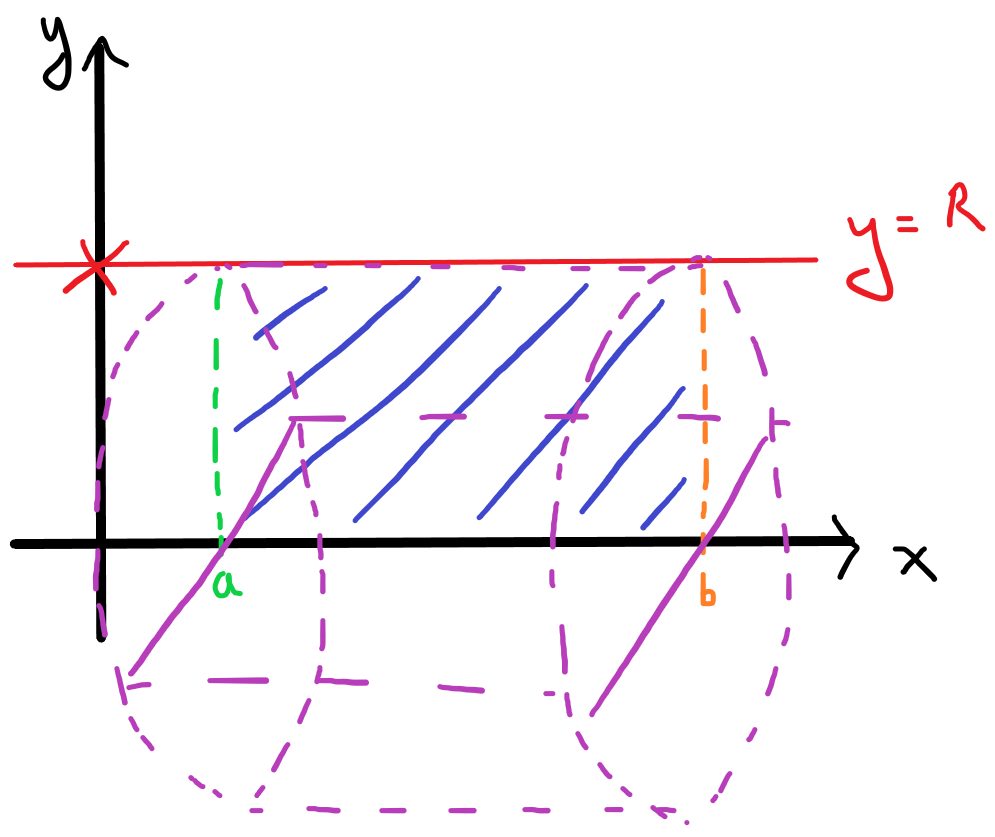
\includegraphics[width=6cm, height=4cm]{assets/ex30-a1-schema.png}
\end{figure}
$$\pi \times \int\limits_a^b (f(x))^2 dx = \pi \times \int\limits_a^b R^2 dx$$ \vspace{0.01cm}

Intéressons-nous à l'intégrale définie \vspace{0.2cm}

\begin{center}
$\displaystyle{\int\limits_a^b R^2 dx = F(b) - F(a)}$ \textit{ssi} $F(x)$ est une primitive de $R^2$ \vspace{0.2cm}

\end{center}

Afin de trouver $F(x)$, il faut résoudre l'intégrale indéfinie \vspace{0.2cm}

$$\int R^2dx = R^2x + c$$ \vspace{0.01cm}

En prenant arbitrairement $F(x)=R^2x$, \vspace{0.2cm}

$$F(b)-F(a) = R^2b-R^2a=R^2\times(b-a)$$ \vspace{0.01cm}

Où $(b-a)$ correspond à la hauteur du cylindre \vspace{0.5cm}

De ce fait,

$$\pi \times \int\limits_a^b R^2 dx = \pi \times R^2 \times h$$

\newpage
%----------------------------------------------------------------------------------------------------------------------------------------
\flushleft \textbf{a.2) Établir la formule permettant de calculer le volume d'une sphère de rayon \textit{R}}

\begin{figure}[h]
    \textit{\caption{}}\vspace{0.2cm}
    \centering
    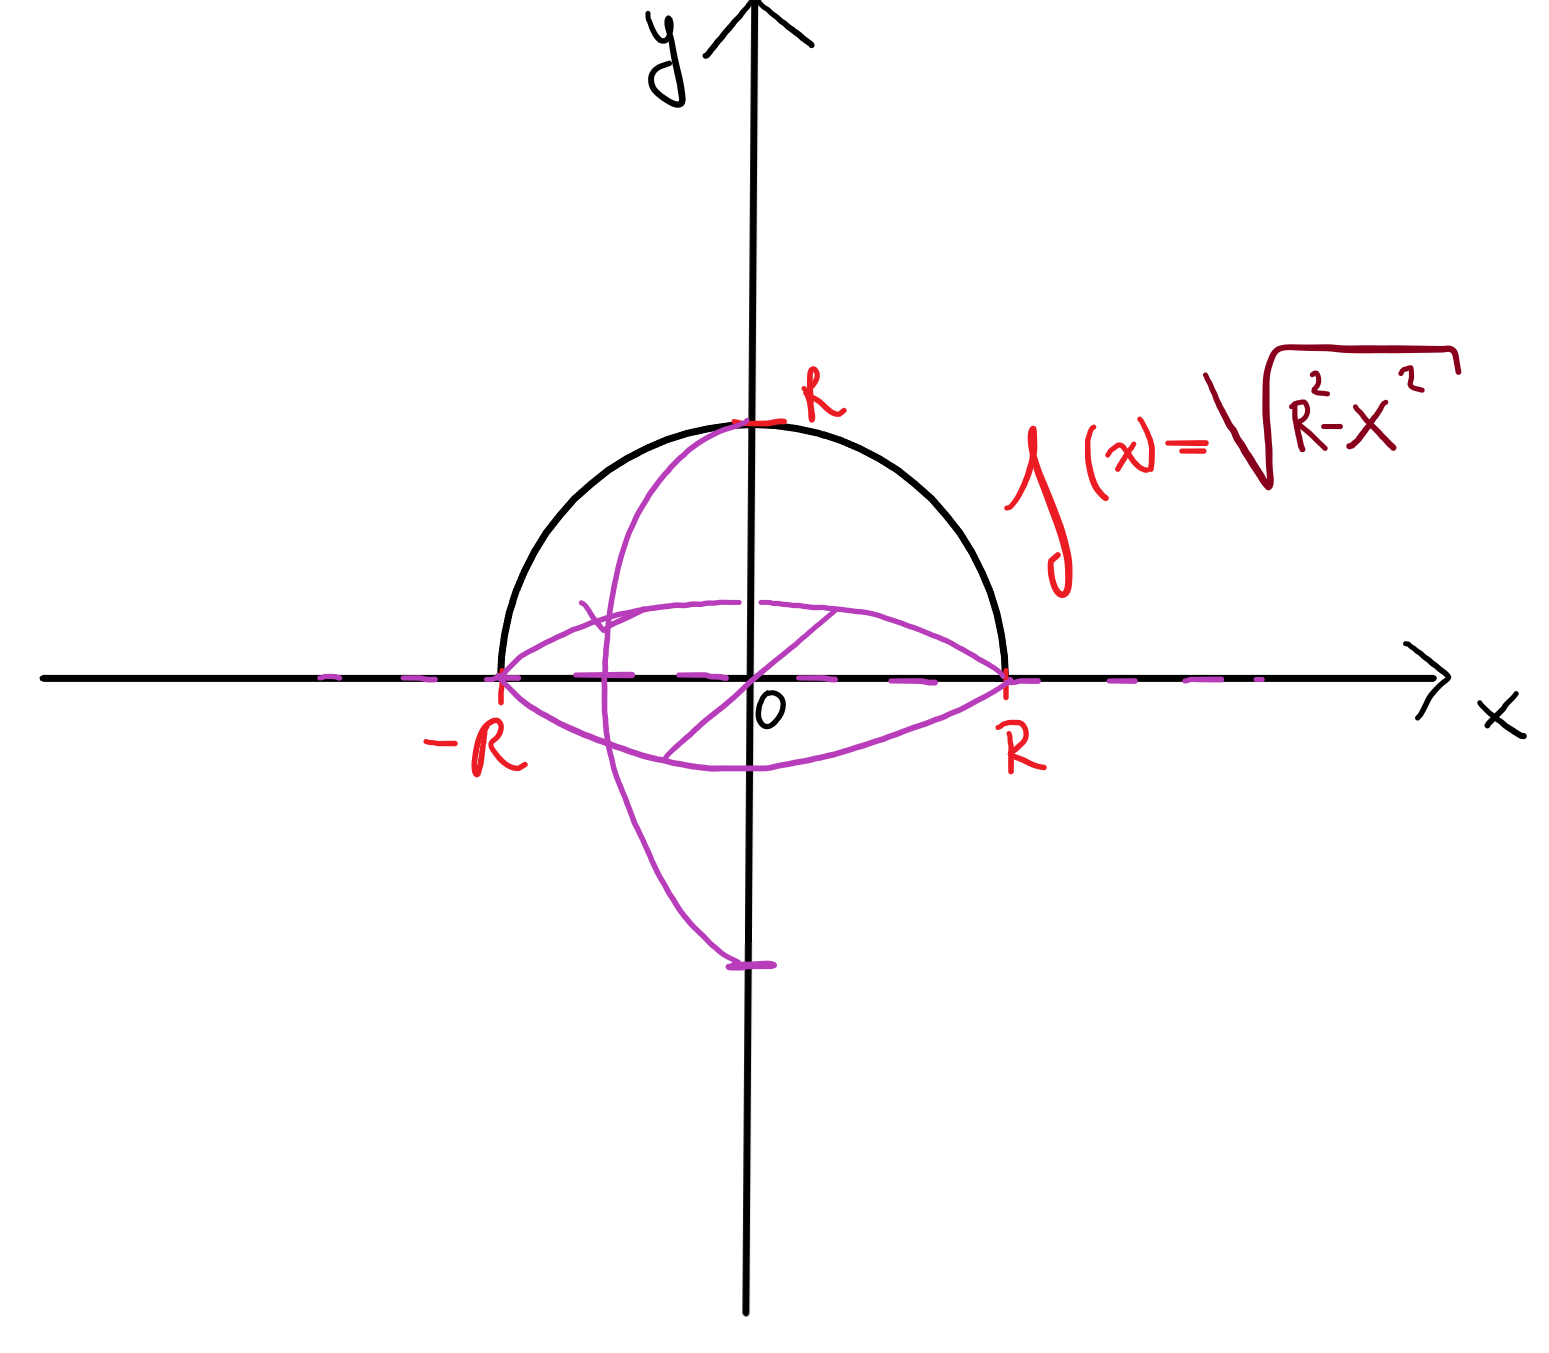
\includegraphics[width=8cm, height=6cm]{assets/ex30-a2-schema.png}
\end{figure}
$$\pi\times\int\limits_a^b(f(x))^2dx = \pi\times\int\limits_{-R}^R[\sqrt{R^2-x^2}]^2dx=\pi\times\int\limits_{-R}^R({R^2-x^2})dx$$\vspace{0.01cm}

Intéressons-nous à l'intégrale définie\vspace{0.2cm}

\begin{center}
$\displaystyle{\int\limits_{-R}^R({R^2-x^2})dx = F(R) - F(-R)}$ \textit{ssi} $F(x)$ est une primitive de $({R^2-x^2})$\vspace{0.2cm}
\end{center}

Afin de trouver $F(x)$, il faut résoudre l'intégrale indéfinie\vspace{0.2cm}

$$\int(R^2-x^2)dx=R^2x-{x^3\over{3}}+c$$\vspace{0.01cm}

En prenant arbitrairement $F(x)=R^2x-{x^3\over{3}}$,\vspace{0.2cm}

$$F(R)-F(-R)=\left[R^3-{R^3\over{3}}\right]-\left[-R^3+{R^3\over{3}}\right]=2R^3-{2R^3\over{3}}={4R^3\over{3}}$$\vspace{0.01cm}

De ce fait,

$$\pi\times\int\limits_{-R}^R({R^2-x^2})dx = \pi\times{4R^3\over{3}}$$

\newpage
%----------------------------------------------------------------------------------------------------------------------------------------
\flushleft \textbf{a.3) Établir la formule permettant de calculer le volume d'un cône droit de rayon \textit{R} et de hauteur \textit{h}}

\begin{figure}[h]
    \textit{\caption{}}\vspace{0.2cm}
    \centering
    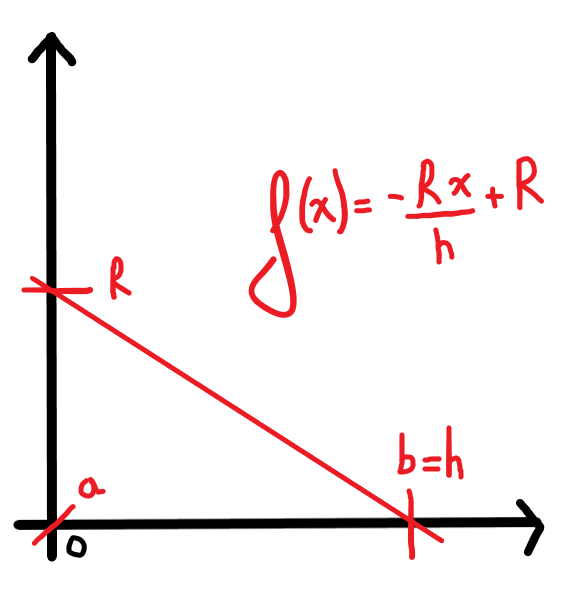
\includegraphics[width=4cm, height=4cm]{assets/ex30-a3-schema.png}
\end{figure}
Trouver la fonction est plus long pour ce cas-ci.
Nous savons que $f(a)=f(0)=R$ et que $f(b)=f(h)=0$\vspace{0.5cm}

La fonction se présente donc sous la forme $\displaystyle{f(x)={y_b-y_a\over{x_b-x_a}}\times{x+R}}$, ce qui revient à $\displaystyle{f(x)={-Rx\over{h}}+R}$\vspace{0.2cm}

$$\pi\times\int\limits_a^b(f(x))^2dx=\pi\times\int\limits_0^h({-Rx\over{h}}+R)^2dx=\pi\times\int\limits_0^h({R^2x^2\over{h^2}}-{2R^2x\over{h}}+R^2)dx$$\vspace{0.01cm}

Intéressons-nous à l'intégrale définie\vspace{0.2cm}

\begin{center}
$\displaystyle{\int\limits_0^h({R^2x^2\over{h^2}}-{2R^2x\over{h}}+R^2)dx = F(h)-F(0})$ \textit{ssi} $F(x)$ est une primitive de $\displaystyle{({R^2x^2\over{h^2}}-{2R^2x\over{h}}+R^2)}$\vspace{0.01cm}
\end{center}

Afin de trouver $F(x)$, il faut résoudre l'intégrale indéfinie\vspace{0.2cm}

$$\int({R^2x^2\over{h^2}}-{2R^2x\over{h}}+R^2)dx={R^2x^3\over{3}h^2}-{R^2x^2\over{h}}+R^2x+c$$\vspace{0.01cm}

En choisissant arbitrairement

$$F(x)={R^2x^3\over{3}h^2}-{R^2x^2\over{h}}+R^2x$$\vspace{0.01cm}

Le calcul de l'intégrale définie devient\vspace{0.2cm}

$$F(h)-F(0)={R^2h^3\over{3}h^2}-{R^2h^2\over{h}}+R^2h={R^2h\over{3}}-R^2h+R^2h={R^2h\over{3}}$$\vspace{0.01cm}

De ce fait,

$$\pi\times\int\limits_0^h({R^2x^2\over{h^2}}-{2R^2x\over{h}}+R^2)dx=\pi\times{R^2h\over{3}}$$

\newpage
%----------------------------------------------------------------------------------------------------------------------------------------
\flushleft \textbf{b. Quel est le rapport des volumes d'un cône droit et d'un cylindre droit de même rayon et de même hauteur}\vspace{0.5cm}

Le rapport est égal à $$\displaystyle{\pi \times R^2 \times h \over{3}} \times {1\over{\pi \times R^2 \times h}}={1\over{3}}$$

%----------------------------------------------------------------------------------------------------------------------------------------
\flushleft \textbf{c. Comparer le volume d'une sphère de rayon \textit{R} et celui du cylindre qui lui est circonscrit}\vspace{0.5cm}

Le volume d'une sphère de rayon R est de $\pi\times{4R^3\over{3}}$\vspace{0.5cm}

Le cylindre qui lui est circonscrit possède, par définition, le même rayon \textit{R}, qui est égal à sa hauteur \textit{h}.\vspace{0.5cm}

Son volume est donc de $\pi \times R^2 \times h=\pi \times R^3$ \vspace{0.5cm}

Le rapport entre le volume de la sphère et le volume du cylindre qui lui est circonscrit est égal à

$$\displaystyle{\pi\times4R^3\over{3}}\times{1\over{\pi \times R^3}}={4\over{3}}$$

%----------------------------------------------------------------------------------------------------------------------------------------
\flushleft \textbf{d. Un tore est un solide de révolution engendré par un cercle tournant autour d'une droite située dans son plan mais ne passant pas par son centre. Montre que le volume V d'un tore engendré par le mouvement d'un cercle de rayon \textit{R} et dont le centre est situé à une distance $a$ de la droite autour de laquelle il tourne, est donné par $V=2a\pi^2 R^2$.}\vspace{0.5cm}

Pour réaliser cet exercice, nous avons besoin des fonctions $f(x)=\sqrt{R^2-x^2}+a$ et $g(x)=-\sqrt{R^2-x^2}+a$

\begin{figure}[h]
    \textit{\caption{Ici, $a=4$ et $R=2$}}\vspace{0.2cm}
    \centering
    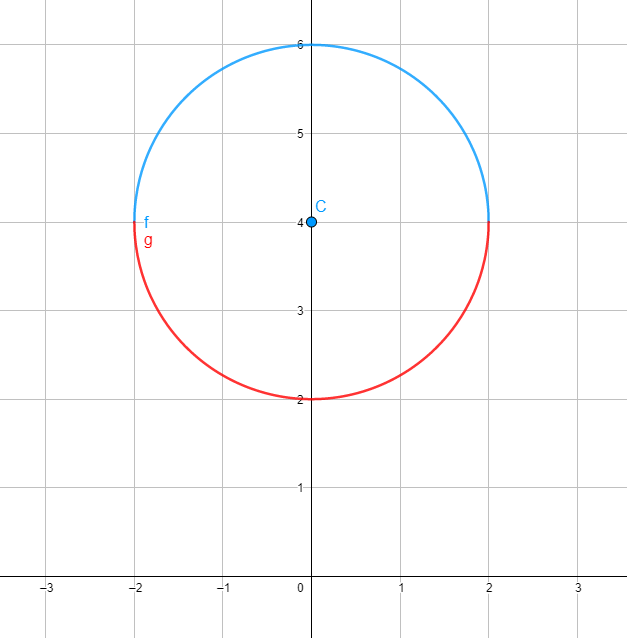
\includegraphics[width=6cm, height=6cm]{assets/ex30-d-schema.png}
\end{figure}


\hspace{0.8cm} Afin de trouver le volume du tore construit par ces deux fonctions, j'ai réalisé le calcul suivant:\vspace{0.2cm}

$$\pi\times\int\limits_{-R}^R(\sqrt{R^2-x^2}+a)^2dx - \pi\times\int\limits_{-R}^R(-\sqrt{R^2-x^2}+a)^2dx$$

$$=\pi\times\left[\left(\int\limits_{-R}^R (a^2+2a\sqrt{R^2-x^2}+R^2-x^2)dx\right)-\left(\int\limits_{-R}^R (a^2-2a\sqrt{R^2-x^2}+R^2-x^2)dx\right)\right]$$

\newpage
%----------------------------------------------------------------------------------------------------------------------------------------
\textbf{1. Recherche des primitives de $f(x)$ et $g(x)$}\vspace{0.5cm}

1.1. Recherche de $F(x)$ \vspace{0.5cm}

\hspace{0.8cm} Passage à l'intégrale indéfinie\vspace{0.2cm}

$$\int (a^2+2a\sqrt{R^2-x^2}+R^2-x^2)dx$$\vspace{0.01cm}

\hspace{0.8cm} Décomposition en somme d'intégrales\vspace{0.2cm}

$$=\int a^2dx + 2a\int(\sqrt{R^2-x^2})dx + \int R^2dx - \int x^2dx$$

$$=a^2x + aR^2\arcsin({x\over{R}}) + ax\sqrt{R^2-x^2} + R^2x - {x^3\over{3}} + c$$

\begin{center}
\hspace{0.8cm} Prenons $\displaystyle{F(x)=a^2x + aR^2\arcsin({x\over{R}}) + ax\sqrt{R^2-x^2} + R^2x - {x^3\over{3}}}$ comme primitive de $f(x)$\vspace{0.2cm}
\end{center}

1.2 Recherche de $G(x)$ \vspace{0.5cm}

\hspace{0.8cm} Passage à l'intégrale indéfinie\vspace{0.2cm}

$$\int (a^2-2a\sqrt{R^2-x^2}+R^2-x^2)dx$$\vspace{0.01cm}

\hspace{0.8cm} Décomposition en somme d'intégrales\vspace{0.2cm}

$$=\int a^2dx - 2a\int(\sqrt{R^2-x^2})dx + \int R^2dx - \int x^2dx$$

$$=a^2x - aR^2\arcsin({x\over{R}}) - ax\sqrt{R^2-x^2} + R^2x - {x^3\over{3}} + c$$

\begin{center}
\hspace{0.8cm} Prenons $\displaystyle{G(x)=a^2x - aR^2\arcsin({x\over{R}}) - ax\sqrt{R^2-x^2} + R^2x - {x^3\over{3}}}$ comme primitive de $g(x)$\vspace{0.2cm}
\end{center}

\textbf{2. Résolution des deux intégrales définies}\vspace{0.5cm}

2.1 Calcul de $F(R)-F(-R)$\vspace{0.2cm}

$$=\left[{2R^3\over{3}}+{aR^2\pi\over{2}}+a^2R\right]-\left[{-2R^3\over{3}}-{aR^2\pi\over{2}} - a^2R\right]$$

$$={4R^3\over{3}}+aR^2\pi + 2a^2R$$\vspace{0.01cm}

2.2. Calcul de $G(R)-G(-R)$\vspace{0.2cm}

$$=\left[{2R^3\over{3}}-{aR^2\pi\over{2}}+a^2R\right]-\left[{-2R^3\over{3}}+{aR^2\pi\over{2}} - a^2R\right]$$

$$={4R^3\over{3}}-aR^2\pi + 2a^2R$$

\newpage
%----------------------------------------------------------------------------------------------------------------------------------------

\textbf{3. Formule finale}\vspace{0.2cm}

$$=\pi\times\left[\left(\int\limits_{-R}^R (a^2+2a\sqrt{R^2-x^2}+R^2-x^2)dx\right)-\left(\int\limits_{-R}^R (a^2-2a\sqrt{R^2-x^2}+R^2-x^2)dx\right)\right]$$

$$=\pi\times\left[\left({4R^3\over{3}}+aR^2\pi + 2a^2R\right)-\left({4R^3\over{3}}-aR^2\pi + 2a^2R\right)\right]$$

$$=\pi\times\left[2aR^2\pi\right]$$

$$=2aR^2\pi^2$$

\end{document}
